\section{Part II: Feature Extraction (for dataset B)}
\subsection{Computing the eigenvectors and eigenvalues using PCA}
The principle component analysis technique was used to reduce the dimensionality of the data to two dimensions. The plot in Figure~\ref{fig:fig2} shows the eigenvalues for each principle component in order of significance. Generally, a "knee" is looked for to determine how many components could be used and still retain a large amount of the variance. Overall, the components tend to decrease fairly smoothly and a knee is not overly evident. We can see a slight drop in variance from component 4 to 5.

\begin{figure}[htb]
 \centering
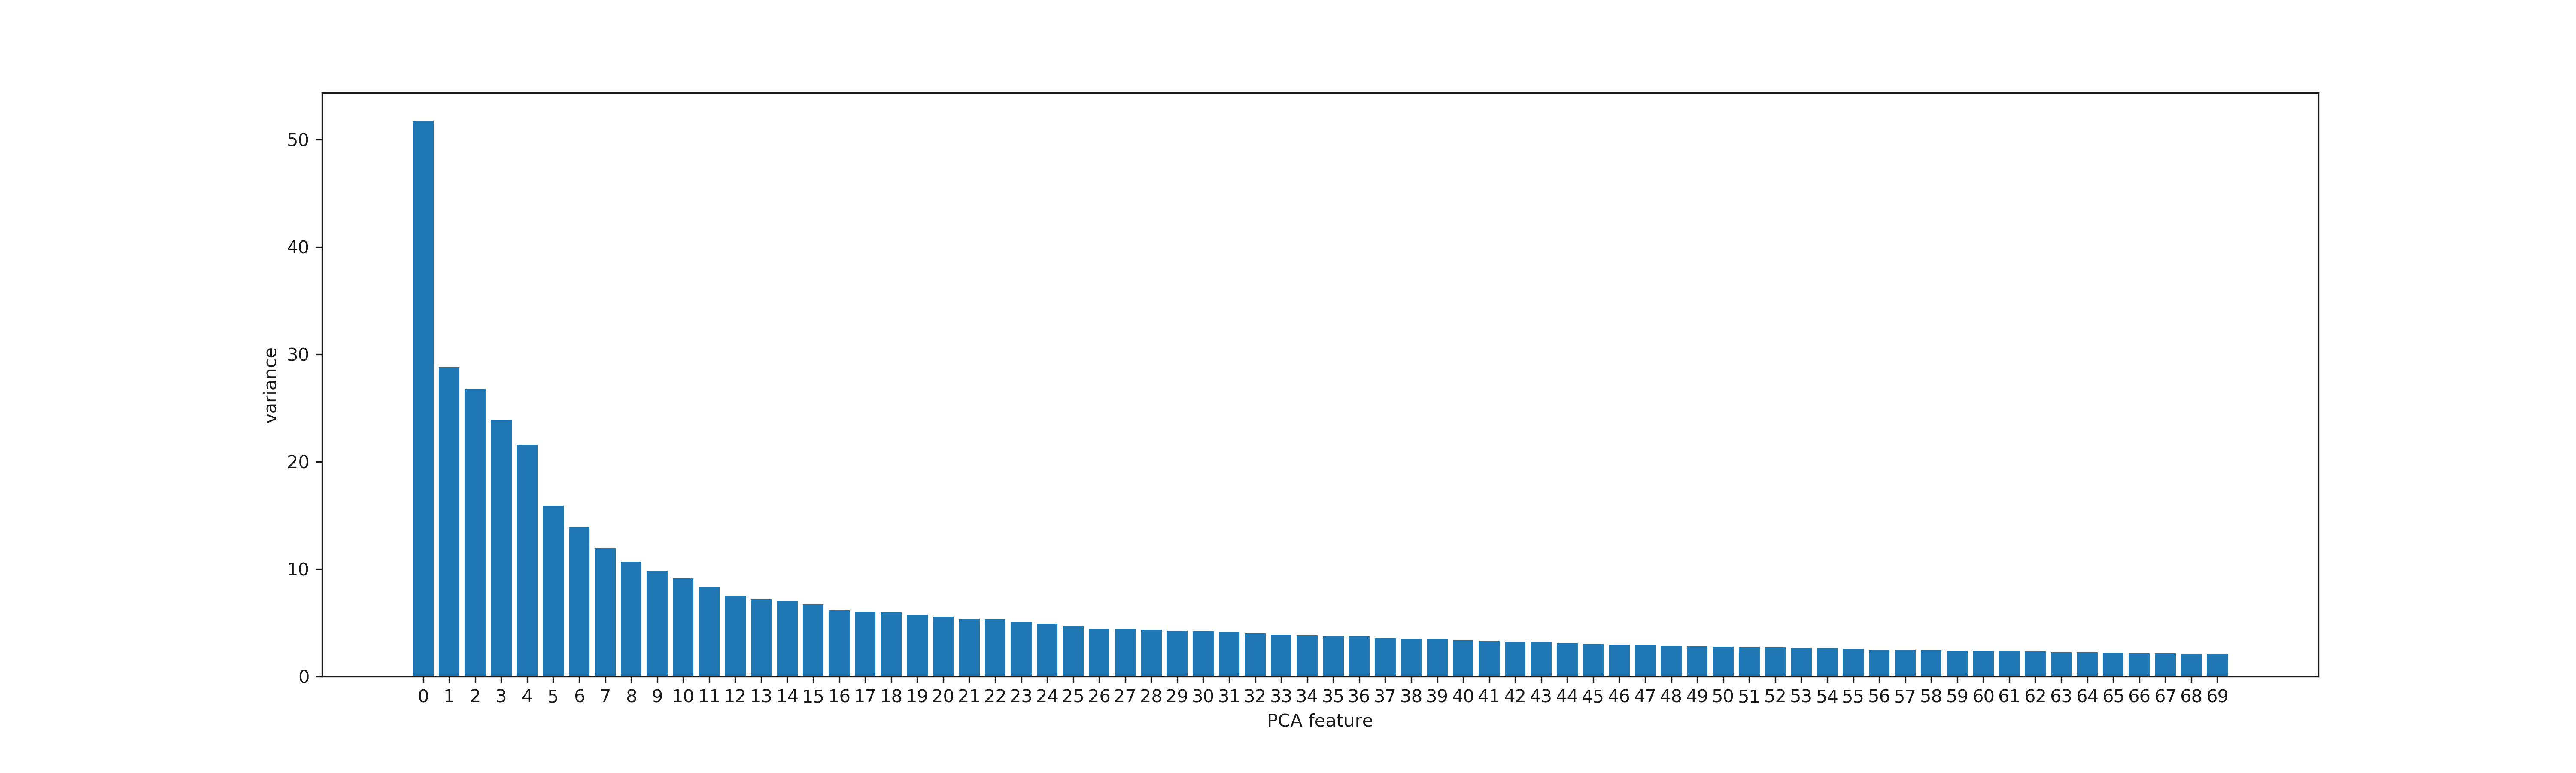
\includegraphics[width=\textwidth]{assignment1/2-1-pcafeatures.png}
\caption{\label{fig:fig2}Scree plot showing the principle components after PCA}
\end{figure}



\clearpage{}
\subsection{2-D plot for the top two PCA's}

Figure~\ref{fig:fig3} .....
\begin{figure}[htb]
 \centering
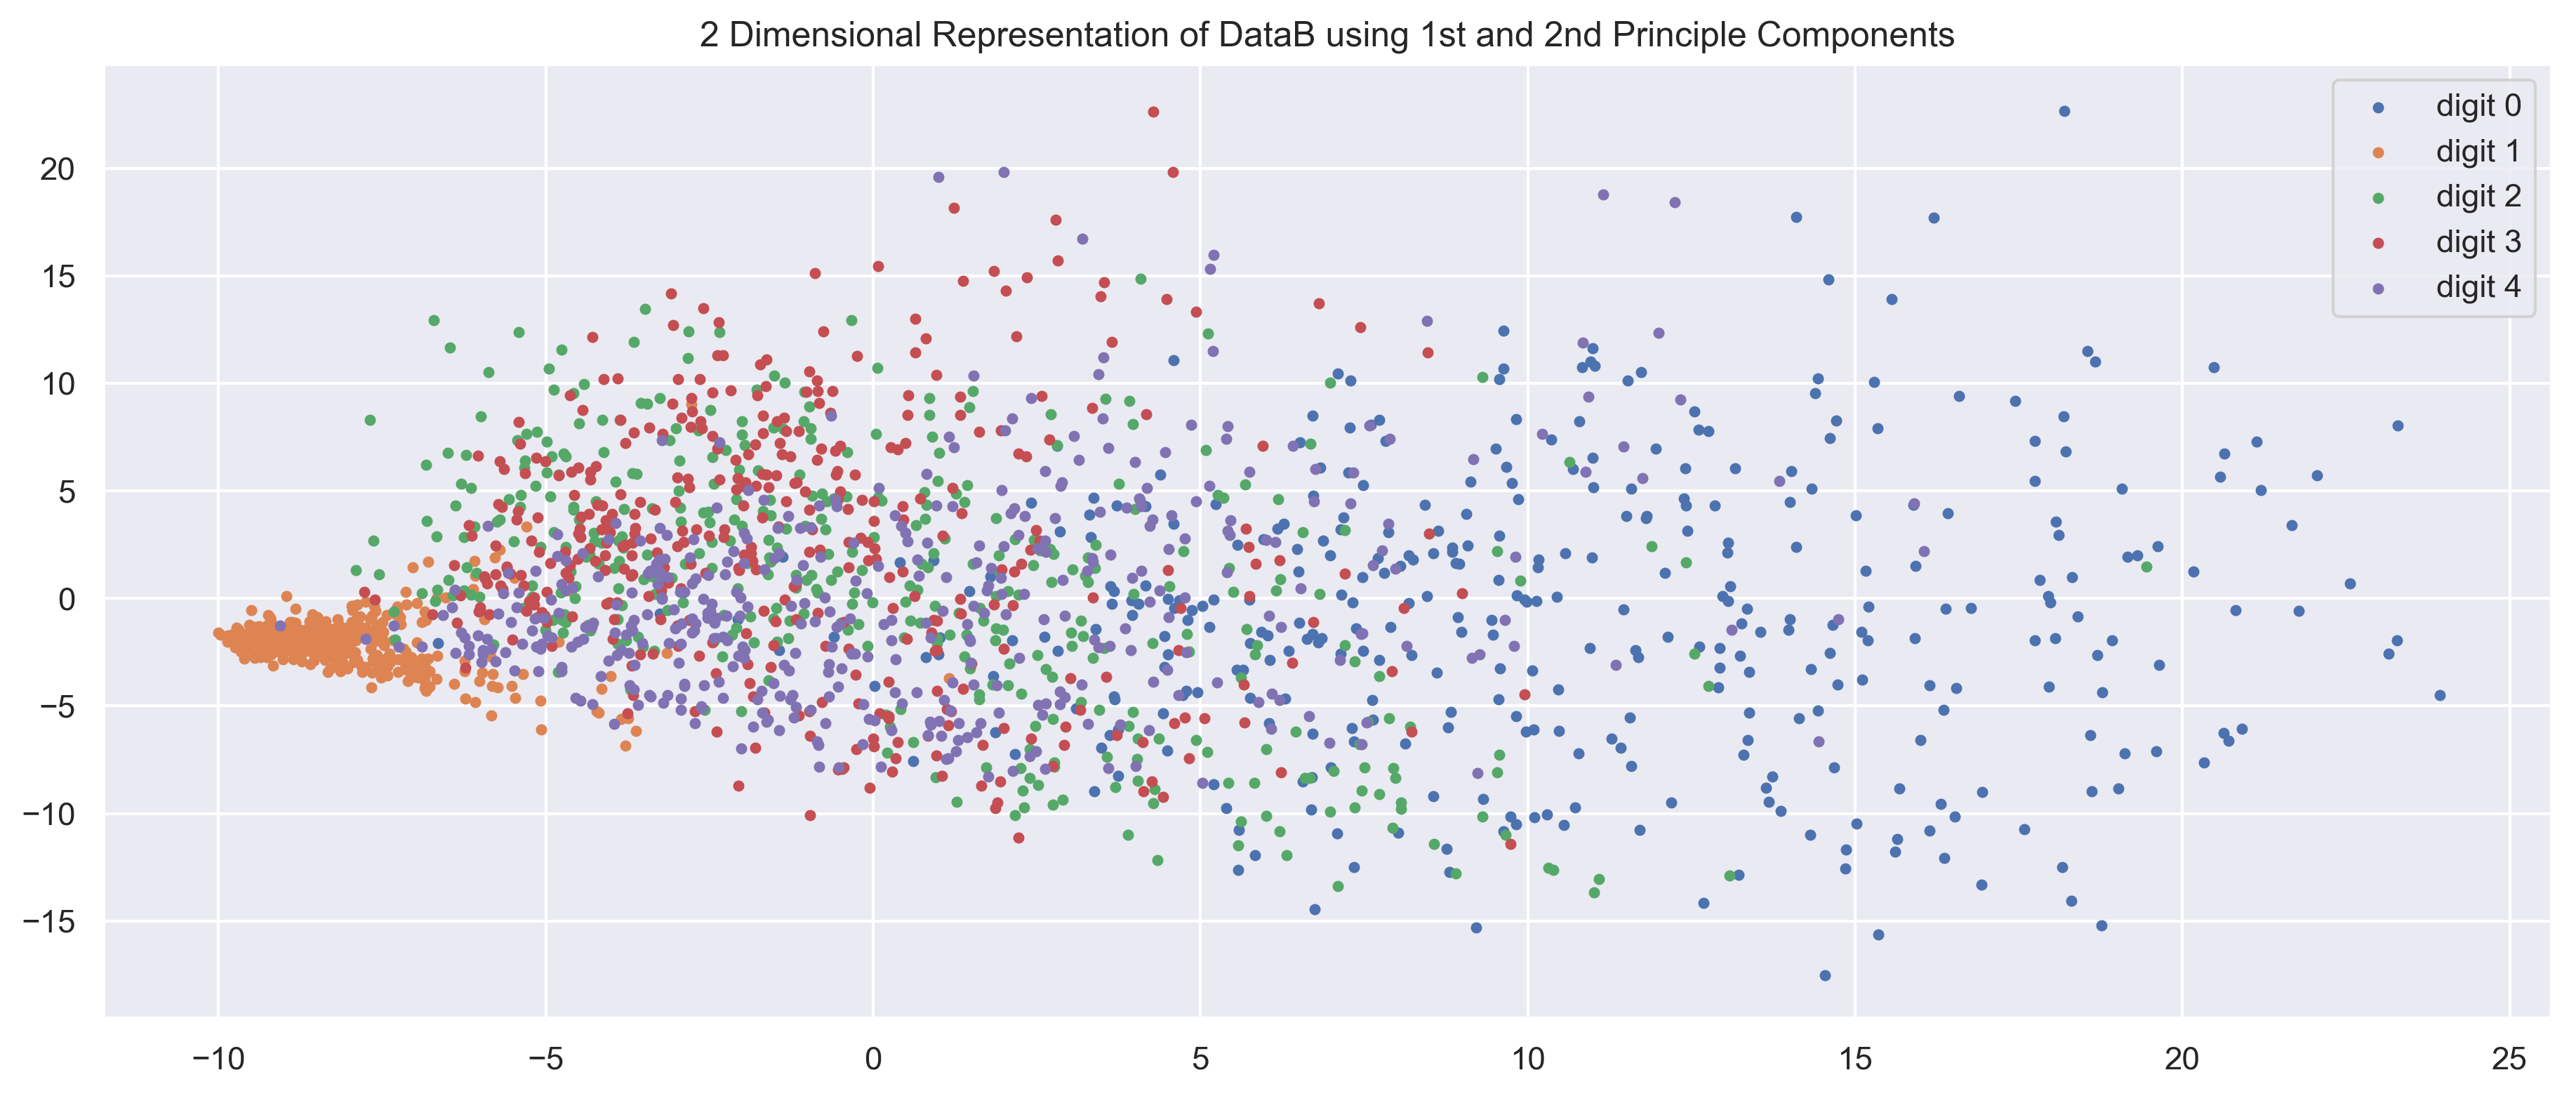
\includegraphics[width=\textwidth]{assignment1/2-2-dimreduction_pca1_2.png}
\caption{\label{fig:fig3}figure caption}
\end{figure}



\clearpage{}
\subsection{2-D plot for the 5th and 6th PCA's}

Figure~\ref{fig:fig4} .....
\begin{figure}[htb]
 \centering
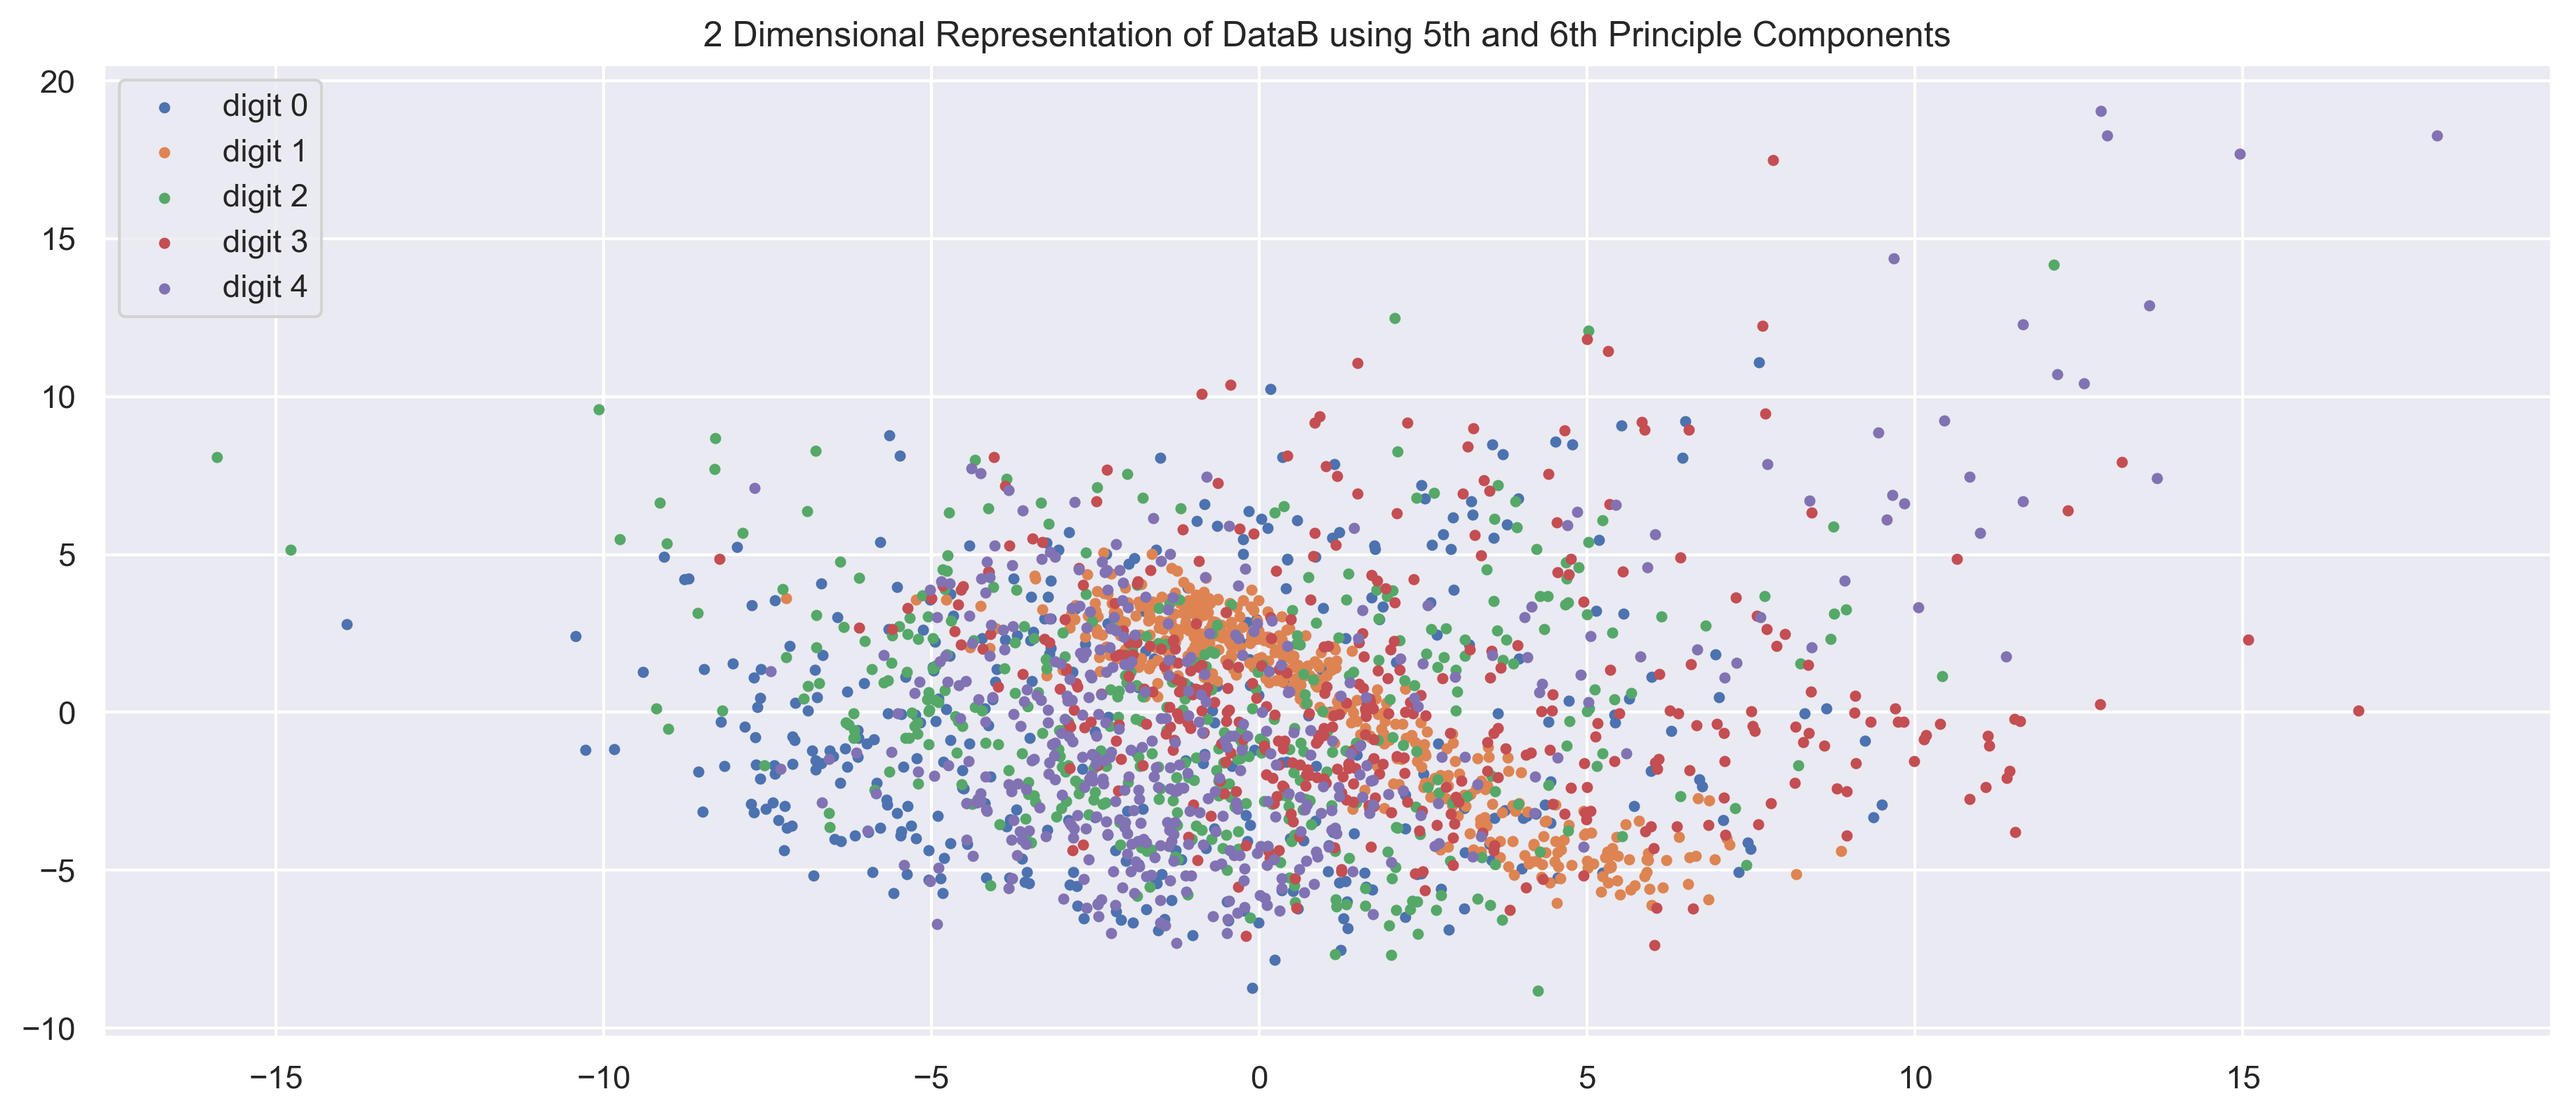
\includegraphics[width=\textwidth]{assignment1/2-3-dimreduction_pca5_6.png}
\caption{\label{fig:fig4}figure caption}
\end{figure}



\clearpage{}
\subsection{Naive Bayes classifier}

Figure~\ref{fig:fig5} .....
\begin{figure}[htb]
 \centering
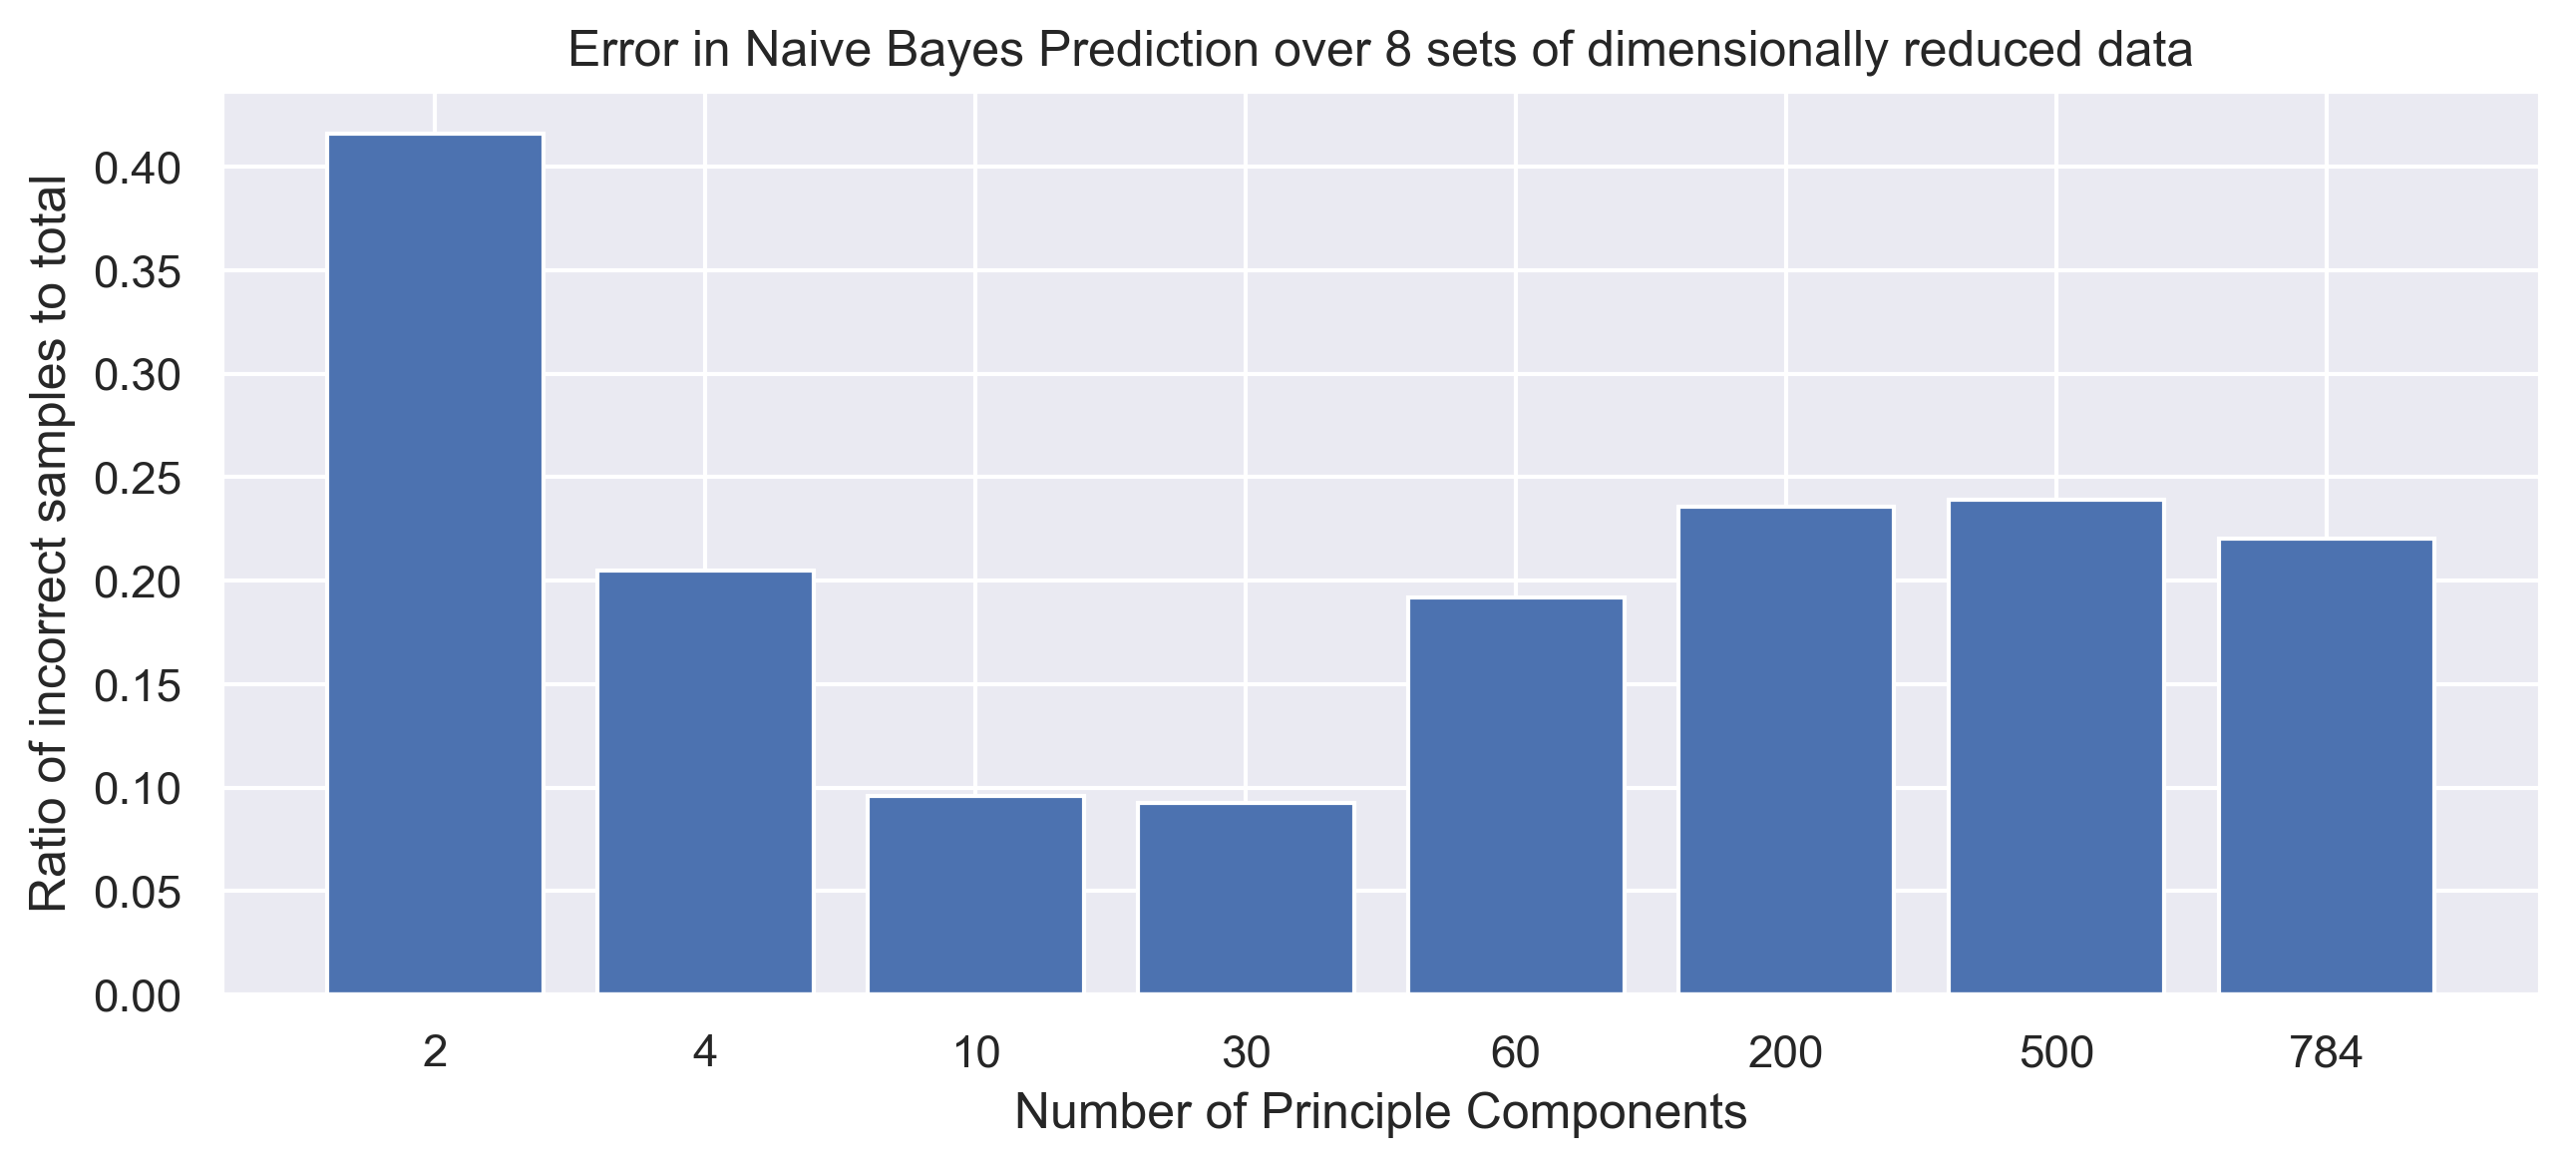
\includegraphics[width=\textwidth]{assignment1/2-4-NBprediction_bar.png}
\caption{\label{fig:fig5}figure caption}
\end{figure}

Figure~\ref{fig:fig6} .....
\begin{figure}[htb]
 \centering
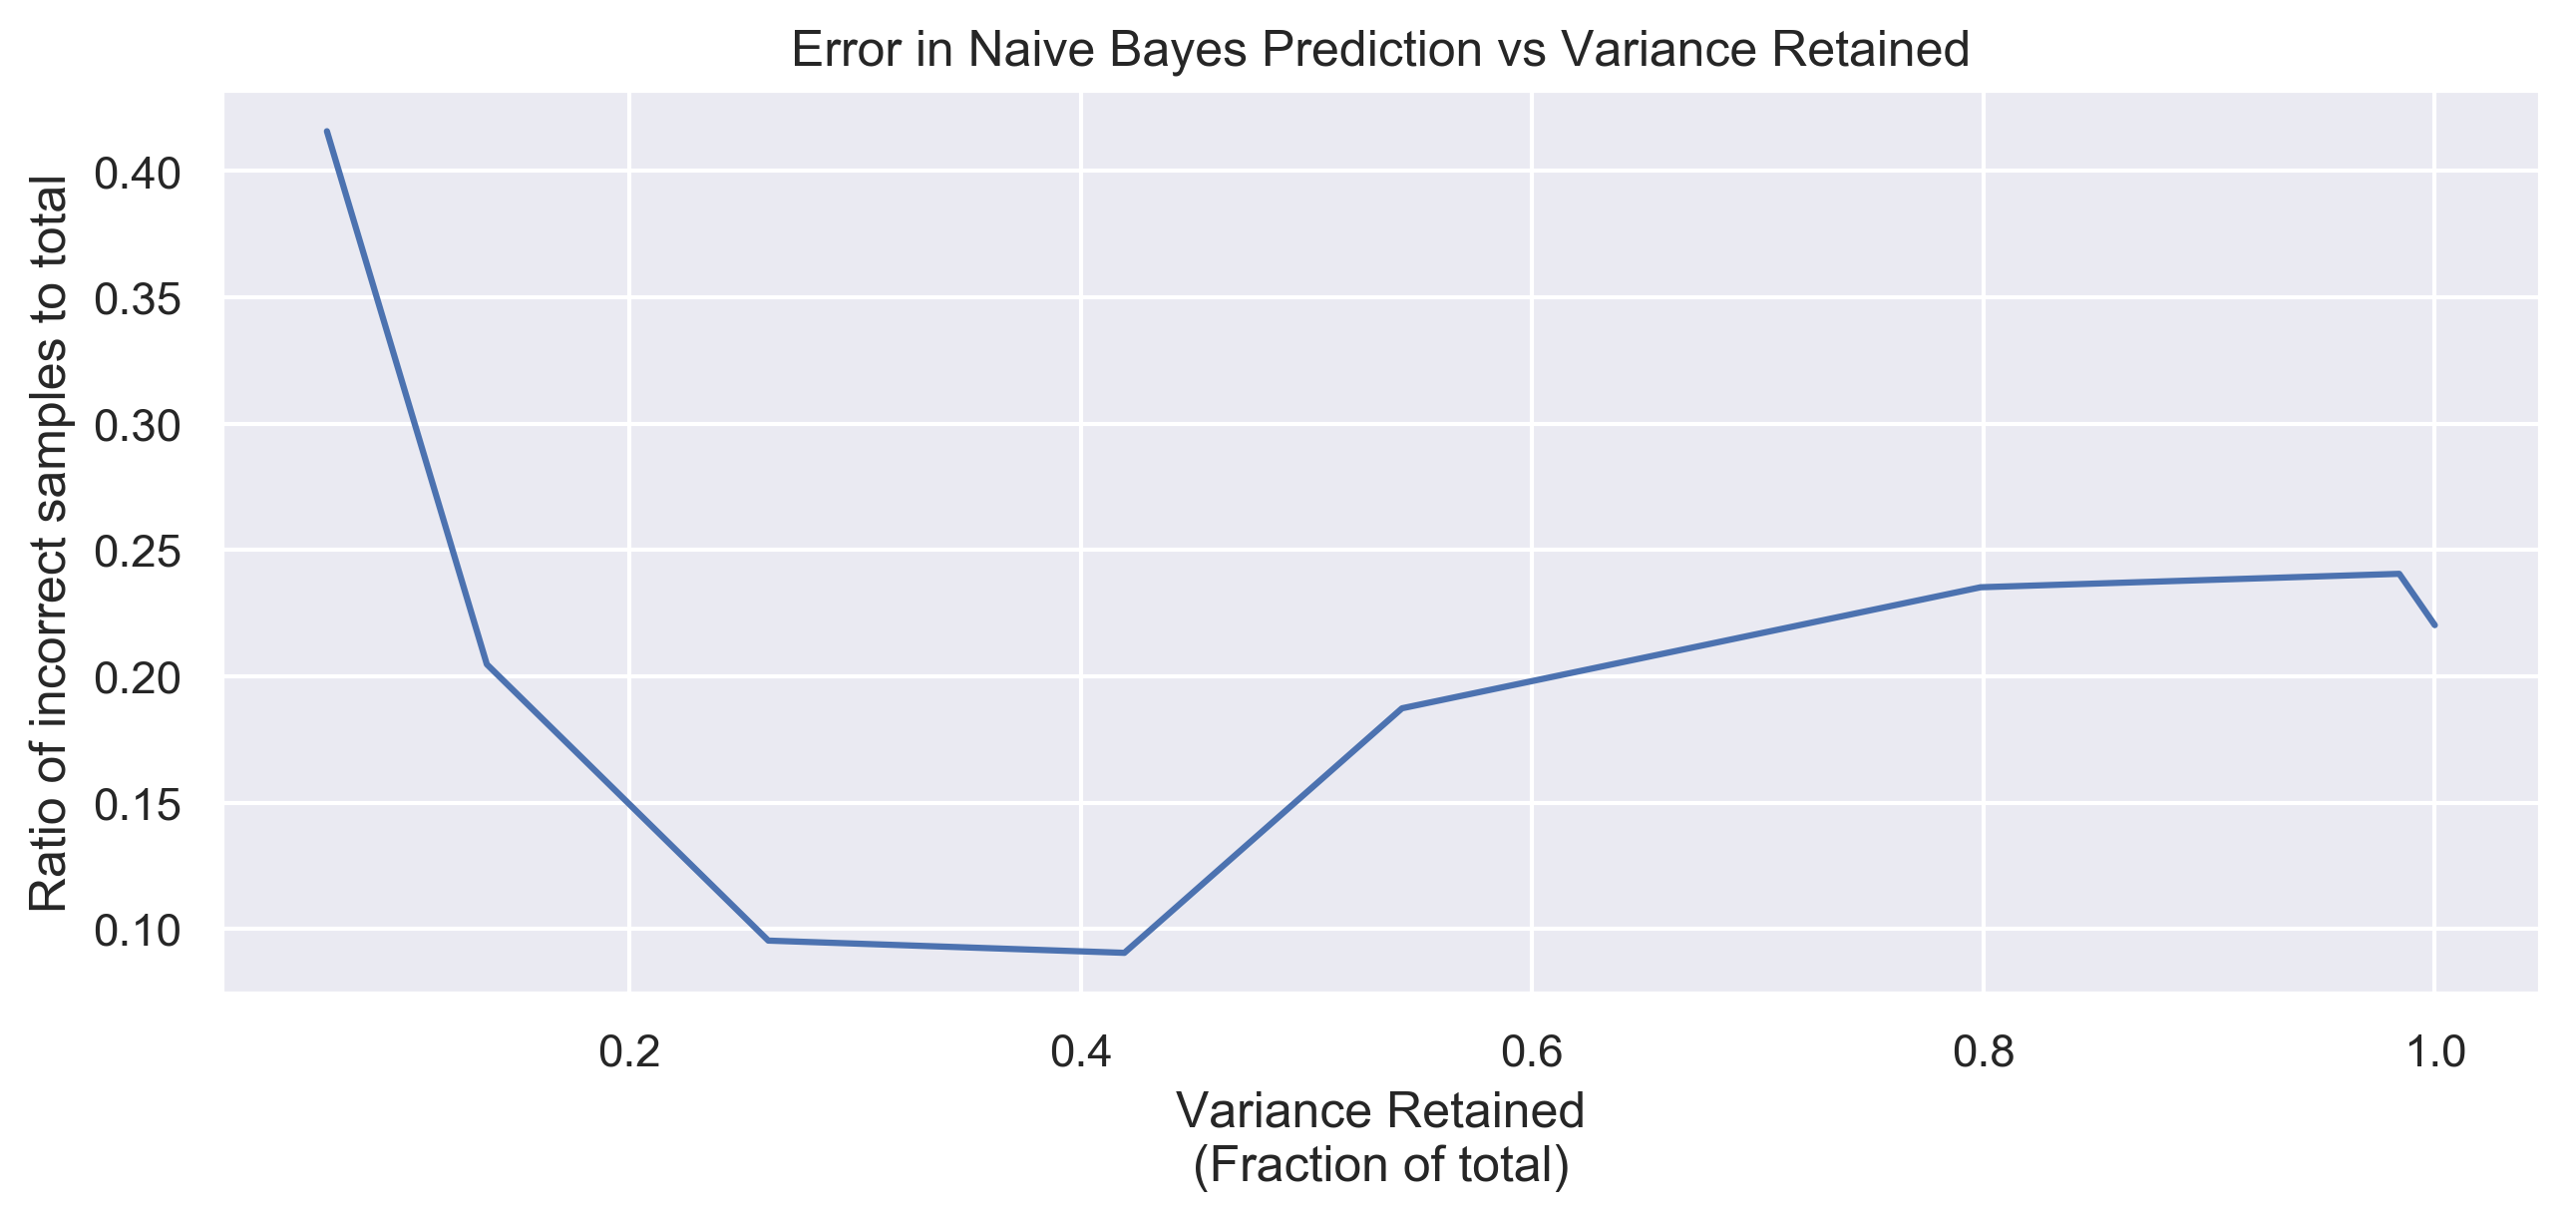
\includegraphics[width=\textwidth]{assignment1/2-4-NBprediction_line.png}
\caption{\label{fig:fig6}figure caption}
\end{figure}



\clearpage{}
\subsection{Linear Discriminant Analysis (LDA)}

Figure~\ref{fig:fig7} .....

\begin{figure}[htb]
 \centering
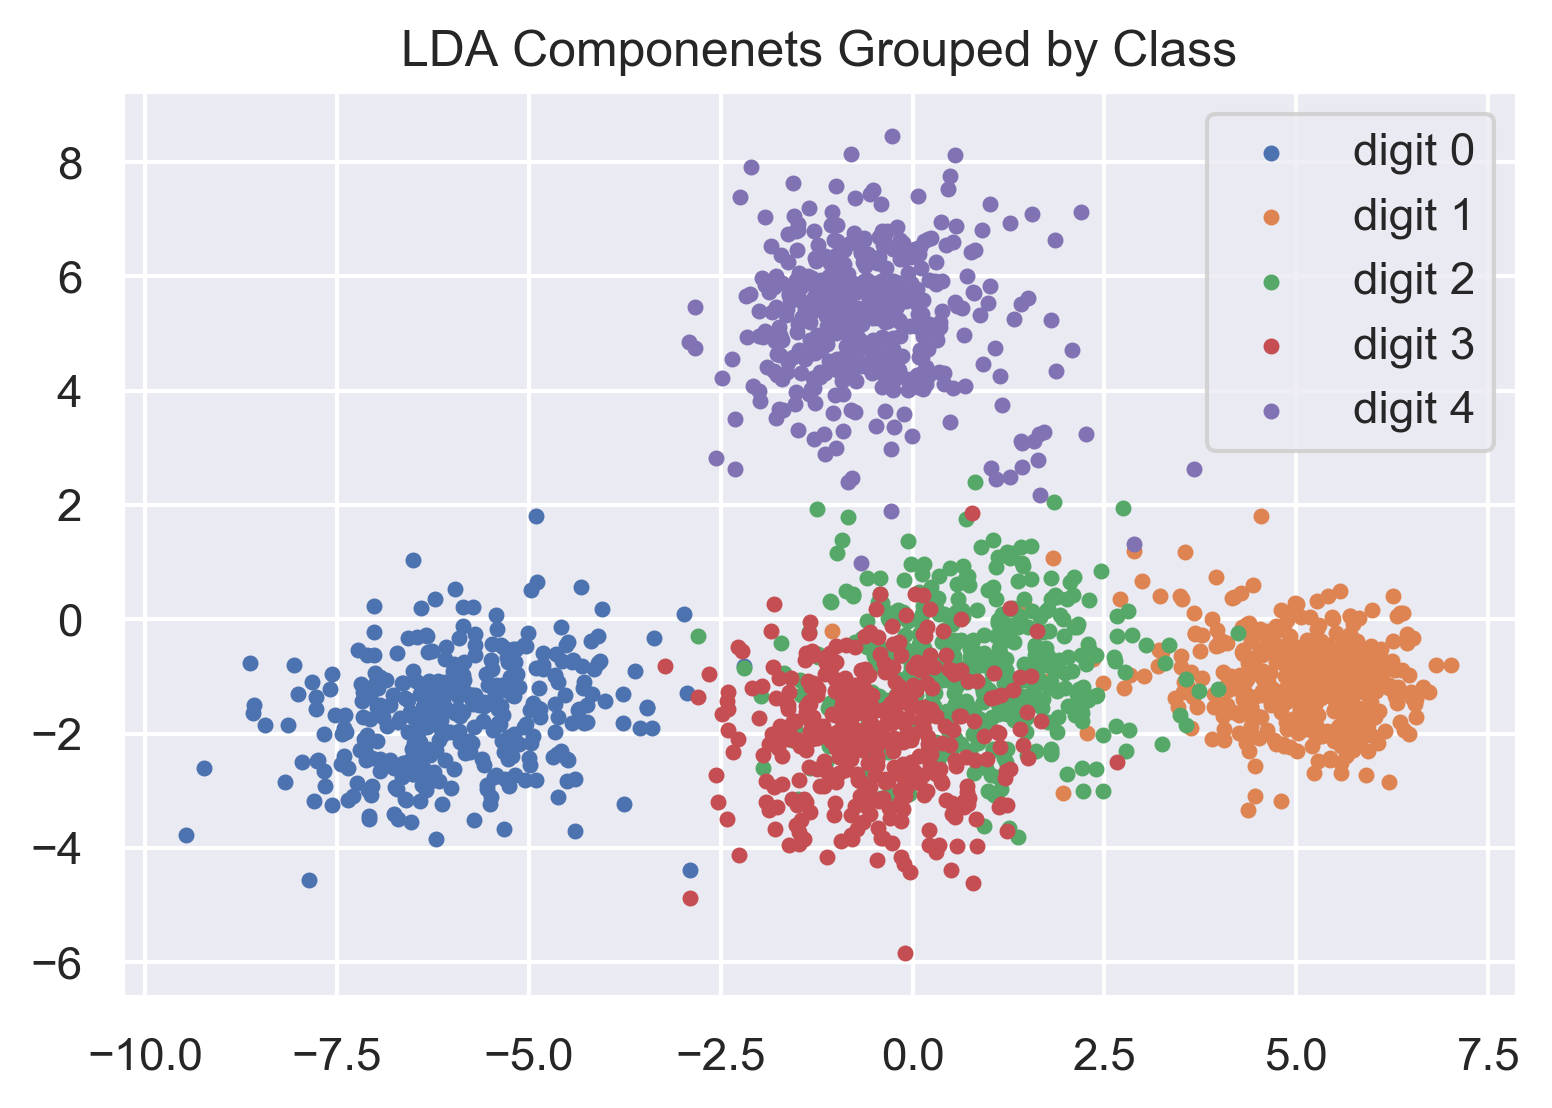
\includegraphics[width=\textwidth]{assignment1/2-5-LDA_dim_reduction.png}
\caption{\label{fig:fig7}figure caption}
\end{figure}